\section{System architecture and artifact admission}
\label{sec:architecture}
ChronoScope separates expensive calculation from evidence delivery. The offline producer reconstructs an admitted series, fits a declared implementation on its observed prefix, scores a separately retained target block, and writes versioned numerical artifacts. Static hosting then serves those artifacts and the browser bundle. There is no active request-time forecasting service behind the published application. The dormant API directory and the OpenAPI components used for type generation do not establish that such a service has been operated or validated. A reproducible offline experiment and a responsive browser view therefore have different execution and acceptance boundaries.

Figure~\ref{fig:report-architecture} shows the responsibilities across these boundaries. Arrows denote artifact dependencies rather than a synchronous prediction API. The browser source is the consumer of admitted artifacts and the owner of current view state.

\begin{figure}[htbp]\centering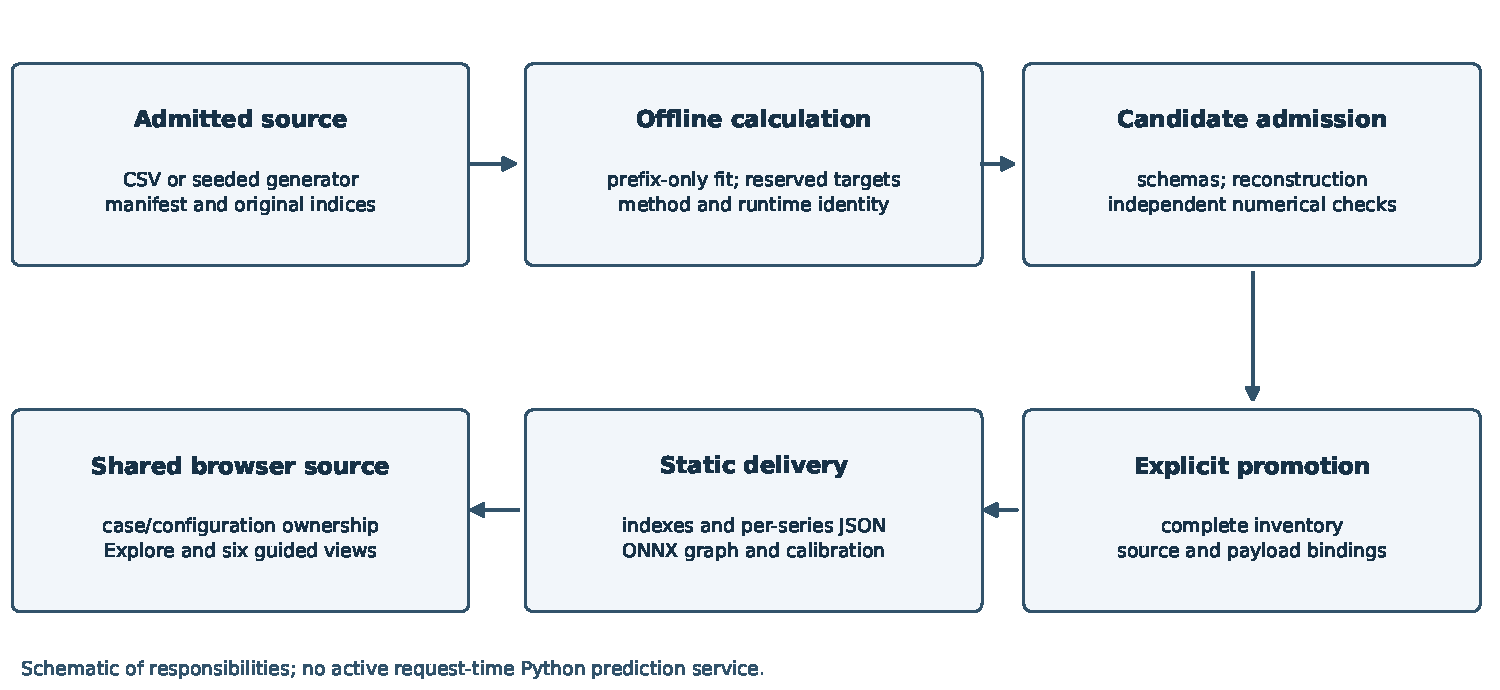
\includegraphics[width=\textwidth]{architecture.pdf}
\caption{Offline calculation, candidate admission, explicit promotion and static browser delivery form separate evidence boundaries; the diagram describes the implemented data flow rather than a request-time forecasting service.}\label{fig:report-architecture}
\end{figure}

The first stage resolves a case identity to its manifest, source description and preprocessing policy. For committed real excerpts, the input is the exact admitted CSV. For a generated mechanism, the case definition and seed determine the observations. Reconstruction checks the original length, the retained display samples and the reserved targets before permitting a comparison. A display trace can be sufficient to draw a picture while being insufficient to reconstruct the fitting series. The second stage supplies the contiguous prefix to the chosen adapter, applying any recorded context cap. Its output contains point and interval columns with the requested horizon. Fitting failures, unavailable dependencies and malformed outputs remain failures or explicit unavailable records; they are not filled by a different algorithm under the requested method name.

The third stage joins forecasts with targets and a historical seasonal scale. It computes scores at the method--case or method--origin level before aggregating at the study's declared unit. This distinction matters: averaging overlapping origins as if they were independent observations would change both the estimand and its uncertainty. The fourth stage constructs delivery documents and compact indexes. Large external-combination records are split by source series, while the complete compressed numerical archive retains the detailed historical selection calculation. The browser index is a navigation aid rather than a replacement for that archive. Independent admission rederives targets, scales, scores and combined paths before a candidate can replace the served documents.

The fifth stage is browser ownership. A single source provider owns the URL-selected case or generator configuration. It fetches the corresponding manifest and required artifacts, rejects subject mismatches, and discards obsolete asynchronous completions. Explore and the six guided views consume this same source. A remembered combination origin may be shown alongside a forecast only when its complete contiguous prefix, length, horizon and targets match; the prefix binding hashes little-endian float64 values. A coincident case name or equal sample count does not satisfy this condition. Generated histories use local computation, and the embedded ONNX path additionally verifies its graph and calibration metadata. These are distinct execution modes, stated in the interface.

Algorithm~\ref{alg:artifact-admission} describes admission as a refusal-oriented sequence. It does not retrain an archived model or certify its scientific accuracy. The existing process also binds stage inputs and payload fingerprints so that a partial case inventory cannot acquire the identity of a complete release. A candidate directory is built and checked before promotion; creating it does not silently overwrite the published data root. This ordering permits independent inspection of a concrete candidate and preserves evidence of a failed attempt.

\begin{algorithm}[htbp]
\caption{Admit a complete forecast artifact candidate against its declared source and execution identities before explicit promotion.}
\label{alg:artifact-admission}
\begin{algorithmic}[1]
\Require Declared case inventory, exact source inputs, implementation bindings, candidate artifacts
\State Refuse missing, extra or duplicated case identities
\For{each declared case}
  \State Validate manifest, trace and analysis against their normative schemas
  \State Reconstruct the complete contiguous source and verify retained samples and targets
  \State Verify the recorded producer and input bindings without rewriting historical identities
  \For{each required forecast path}
    \State Check horizon, finite values, ordered interval columns and method identity
    \State Recompute scores using the declared targets and historical scale
    \State Refuse disagreement beyond the recorded numerical tolerance
  \EndFor
  \State Verify optional study links against the complete prefix and target binding
\EndFor
\State Check index references, expected inventory and candidate payload fingerprints
\State Report an admitted candidate; retain explicit promotion as a separate operation
\end{algorithmic}
\end{algorithm}

This architecture supports independent numerical checks without making every browser request repeat model training. It also creates a responsibility to distinguish a stored result from a new execution. The archived-path comparison reuses some historical predictions, the fresh comparison executes the full roster again, and the external combination study has its own inputs and aggregation. Their schemas, provenance and consumer labels retain these distinctions. A successful schema check cannot substitute for a source reconstruction, and a successful reconstruction cannot establish representative sampling or pretraining independence. The report's evidence claims remain attached to the relevant stage rather than inherited from successful delivery.
